\documentclass[portrait,paperwidth=84.1cm,paperheight=118.9cm]{baposter}

\usepackage{mathtools}
\usepackage{calc}
\usepackage{graphicx}
\usepackage{amsmath}
\usepackage{amssymb}
\usepackage{relsize}
\usepackage{multirow}
\usepackage{rotating}
\usepackage{bm}
\usepackage{url}
\usepackage{mathpazo}
\usepackage{multicol}

\usepackage{tcolorbox}
\tcbuselibrary{listings, skins}
\usepackage{listings}
\usepackage{verbatim}
\usepackage{xcolor}  % Para colores (opcional)
\usepackage{pythontex}

%%%%%%%%%%%%%% los puse yo?
\usepackage{latexsym}
\usepackage{tikz}
\usepackage{arydshln}
\usetikzlibrary{positioning, shapes}
\usepackage[spanish]{babel}
\usepackage{enumitem}
\def\R{{\mathbb {R}}}
\def\div{\operatorname{\text{div}}}
\def\N{{\mathbb {N}}}
\def\A{{\mathcal{A}}}
%%%%%%%%%%%%%%

\usepackage{times}
\usepackage{helvet}
\usepackage{bookman}
\usepackage{palatino} % Font

\lstset{
  language=Python,
  basicstyle=\ttfamily\small,
  keywordstyle=\color{blue},
  commentstyle=\color{gray},
  stringstyle=\color{orange},
  showstringspaces=false,
  frame=single,
  breaklines=true
}

\newcommand{\captionfont}{\footnotesize}

\graphicspath{{images/}{../images/}}
\usetikzlibrary{calc}

%%%%%%%%%%%%%%%%%%%%%%%%%%%%%%%%%%%%%%%%%%%%%%%%%%%%%%%%%%%%%%%%%%%%%%%%%%%%%%%%
%%%% Some math symbols used in the text
%%%%%%%%%%%%%%%%%%%%%%%%%%%%%%%%%%%%%%%%%%%%%%%%%%%%%%%%%%%%%%%%%%%%%%%%%%%%%%%%

%%%%%%%%%%%%%%%%%%%%%%%%%%%%%%%%%%%%%%%%%%%%%%%%%%%%%%%%%%%%%%%%%%%%%%%%%%%%%%%%
% Multicol Settings
%%%%%%%%%%%%%%%%%%%%%%%%%%%%%%%%%%%%%%%%%%%%%%%%%%%%%%%%%%%%%%%%%%%%%%%%%%%%%%%%
\setlength{\columnsep}{1.5em}
\setlength{\columnseprule}{0mm}

%%%%%%%%%%%%%%%%%%%%%%%%%%%%%%%%%%%%%%%%%%%%%%%%%%%%%%%%%%%%%%%%%%%%%%%%%%%%%%%%
% Save space in lists. Use this after the opening of the list
%%%%%%%%%%%%%%%%%%%%%%%%%%%%%%%%%%%%%%%%%%%%%%%%%%%%%%%%%%%%%%%%%%%%%%%%%%%%%%%%
\newcommand{\compresslist}{%
\setlength{\itemsep}{1pt}%
\setlength{\parskip}{0pt}%
\setlength{\parsep}{0pt}%
}

%%%%%%%%%%%%%%%%%%%%%%%%%%%%%%%%%%%%%%%%%%%%%%%%%%%%%%%%%%%%%%%%%%%%%%%%%%%%%%
%%% Begin of Document
%%%%%%%%%%%%%%%%%%%%%%%%%%%%%%%%%%%%%%%%%%%%%%%%%%%%%%%%%%%%%%%%%%%%%%%%%%%%%%

\begin{document}

%%%%%%%%%%%%%%%%%%%%%%%%%%%%%%%%%%%%%%%%%%%%%%%%%%%%%%%%%%%%%%%%%%%%%%%%%%%%%%
%%% Here starts the poster
%%%---------------------------------------------------------------------------
%%% Format it to your taste with the options
%%%%%%%%%%%%%%%%%%%%%%%%%%%%%%%%%%%%%%%%%%%%%%%%%%%%%%%%%%%%%%%%%%%%%%%%%%%%%%
% Define some colors

%\definecolor{lightblue}{cmyk}{0.83,0.24,0,0.12}
\definecolor{lightblue}{rgb}{0.145,0.6666,1}
\definecolor{rojo}{RGB}{216, 36, 36}
\definecolor{rojoobscuro}{RGB}{174, 30, 30}
\definecolor{celeste}{RGB}{71, 148, 227}
\definecolor{celesteosbscuro}{RGB}{71, 148, 227}
\definecolor{lila}{rgb}{.6,.5,0.9}
%%
\begin{poster}%
  % Poster Options
  {
  % Show grid to help with alignment
  grid=false,
  %number of columns
  columns=2,
  % Column spacing
  colspacing=1em,
  % Color style
  bgColorOne=white,
  bgColorTwo=white,
  borderColor=celesteosbscuro,
  headerColorOne=black,
  headerColorTwo=celeste,
  headerFontColor=white,
  boxColorOne=white,
  boxColorTwo=blue, %celeste,
  % Format of textbox
  % textborder=roundedleft,
  textborder=none,
  % Format of text header
  eyecatcher=true,
  % headerborder=closed,
  headerborder=none,
  headerheight=0.1\textheight,
%  textfont=\sc, An example of changing the text font
  headershape=roundedright,
  headershade=shadelr,
  headerfont=\Large\bf\textsc, %Sans Serif
  textfont={\setlength{\parindent}{1.5em}},
  boxshade=plain,
%  background=shade-tb,
  background=plain,
  linewidth=2pt
  }
  % Logo 1
  {
  
\includegraphics[width=90 pt]{logo.jpg}
  }
  % Title
  {\textsc{Investigathon - Modelos de Lenguaje}}
  % Authors
  {\Large Bogetti Gianfranco y  Salmun Daniel\\}
  
%%%%%%%%%%%%%%%%%%%%%%%%%%%%%%%%%%%%%%%%%%%%%%%%%%%%%%%%%%%%%%%%%%%%%%%%%%%%%%
%%% Now define the boxes that make up the poster
%%%---------------------------------------------------------------------------
%%% Each box has a name and can be placed absolutely or relatively.
%%% The only inconvenience is that you can only specify a relative position
%%% towards an already declared box. So if you have a box attached to the
%%% bottom, one to the top and a third one which should be in between, you
%%% have to specify the top and bottom boxes before you specify the middle
%%% box.
%%%%%%%%%%%%%%%%%%%%%%%%%%%%%%%%%%%%%%%%%%%%%%%%%%%%%%%%%%%%%%%%%%%%%%%%%%%%%%

\headerbox{Introducción}{name=intro,column=0}
{
  La eficiencia de los modelos de \textit{LLM} ha impulsado su uso como \textbf{asistentes conversacionales}. Sin embargo, una de las limitaciones de las \textit{LLMs} es que tienen un límite de contexto. Por lo tanto, en los últimos años se han desarrollado sistemas de \textbf{\textit{Retrieval-Augmented Generation (RAG)}}[1], que combinan recuperación y generación para enriquecer la entrada a la \textit{LLM} en base a una fuente de conocimiento.

  En este trabajo, presentamos un sistema de \textit{RAG} para el dataset \textit{LongMemEval}[2], \textbf{restringiendo los modelos de \textit{LLM} a no más de 4B parámetros}, con el objetivo de posibilitar su ejecución local en dispositivos personales, preservando así privacidad, coste y latencia.
}


\headerbox{Dataset}{name=dataset,column=0, below=intro}
{
Los conjuntos de datos utilizados en este trabajo fueron los de \textit{LongMemEval} y los de \textit{Investigathon}, siendo este último una variación acotada del primero. Estos datasets tienen como propósito \textbf{evaluar la capacidad de los modelos para mantener y utilizar memoria a largo plazo en conversaciones multi-sesión}. Tienen distintas tipos de preguntas que se pueden categorizar en los siguientes grupos:

\begin{center}
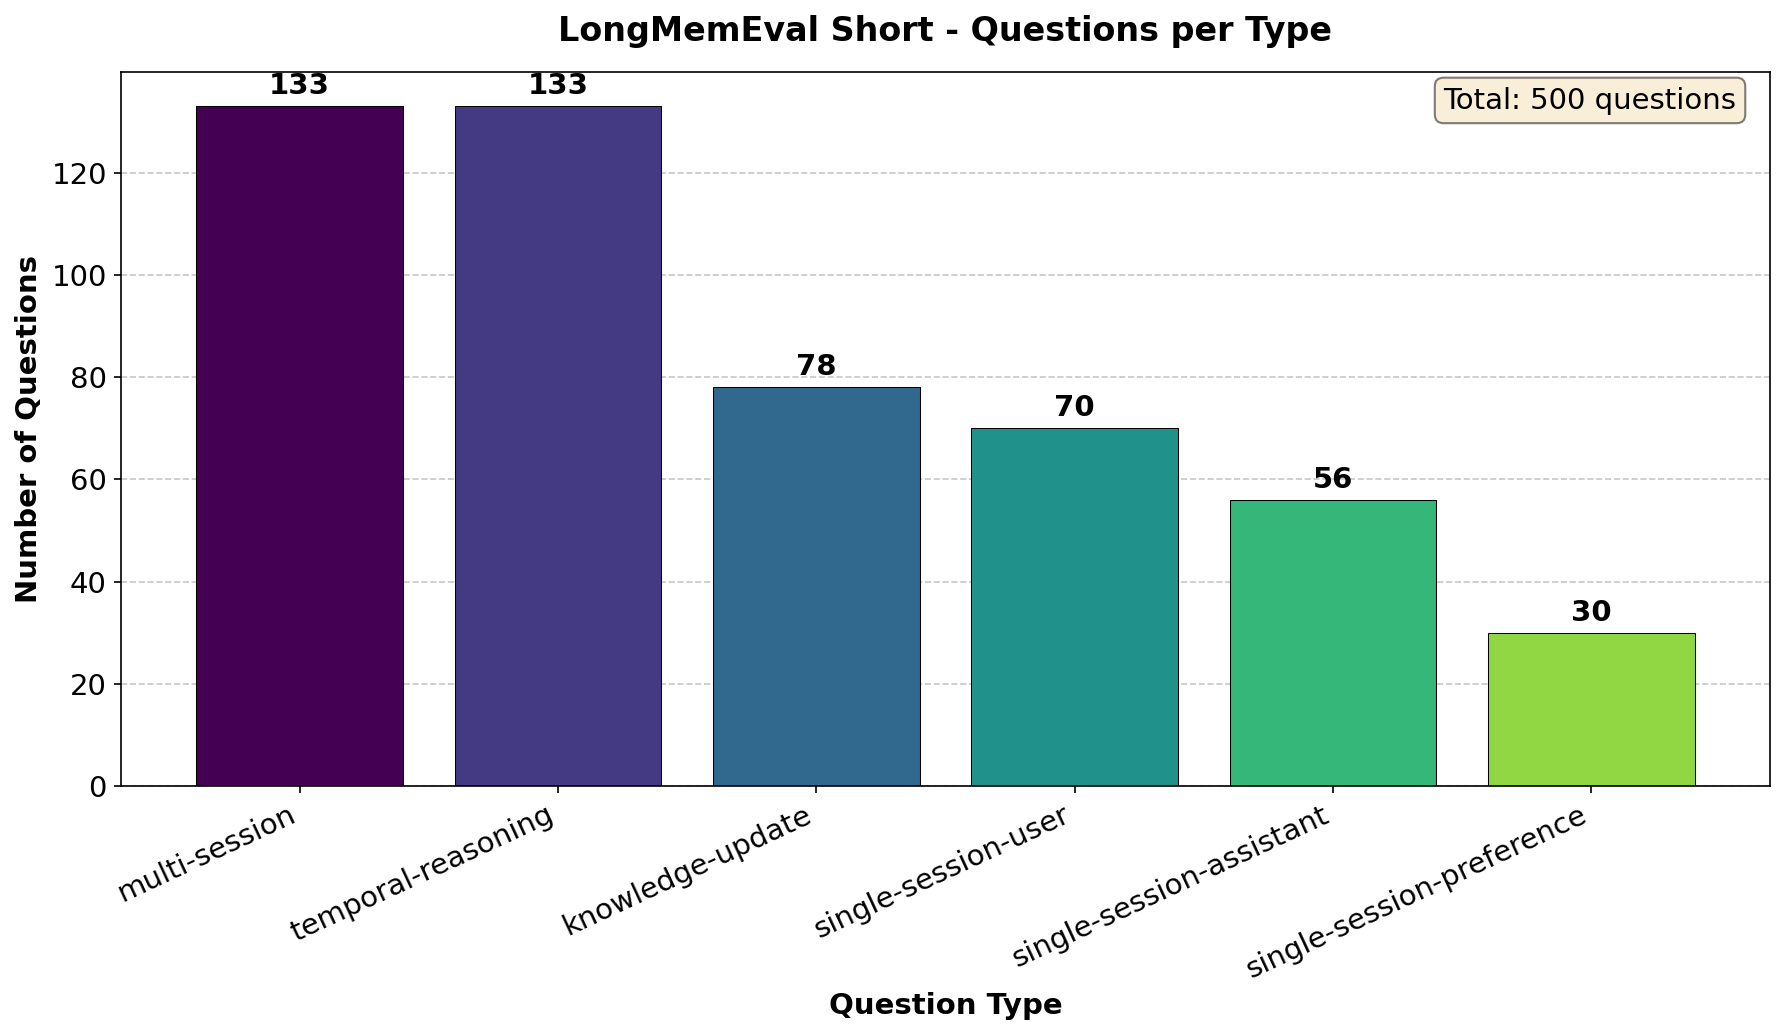
\includegraphics[width=0.48\columnwidth]{images/question_types_longmemeval_short.png} 
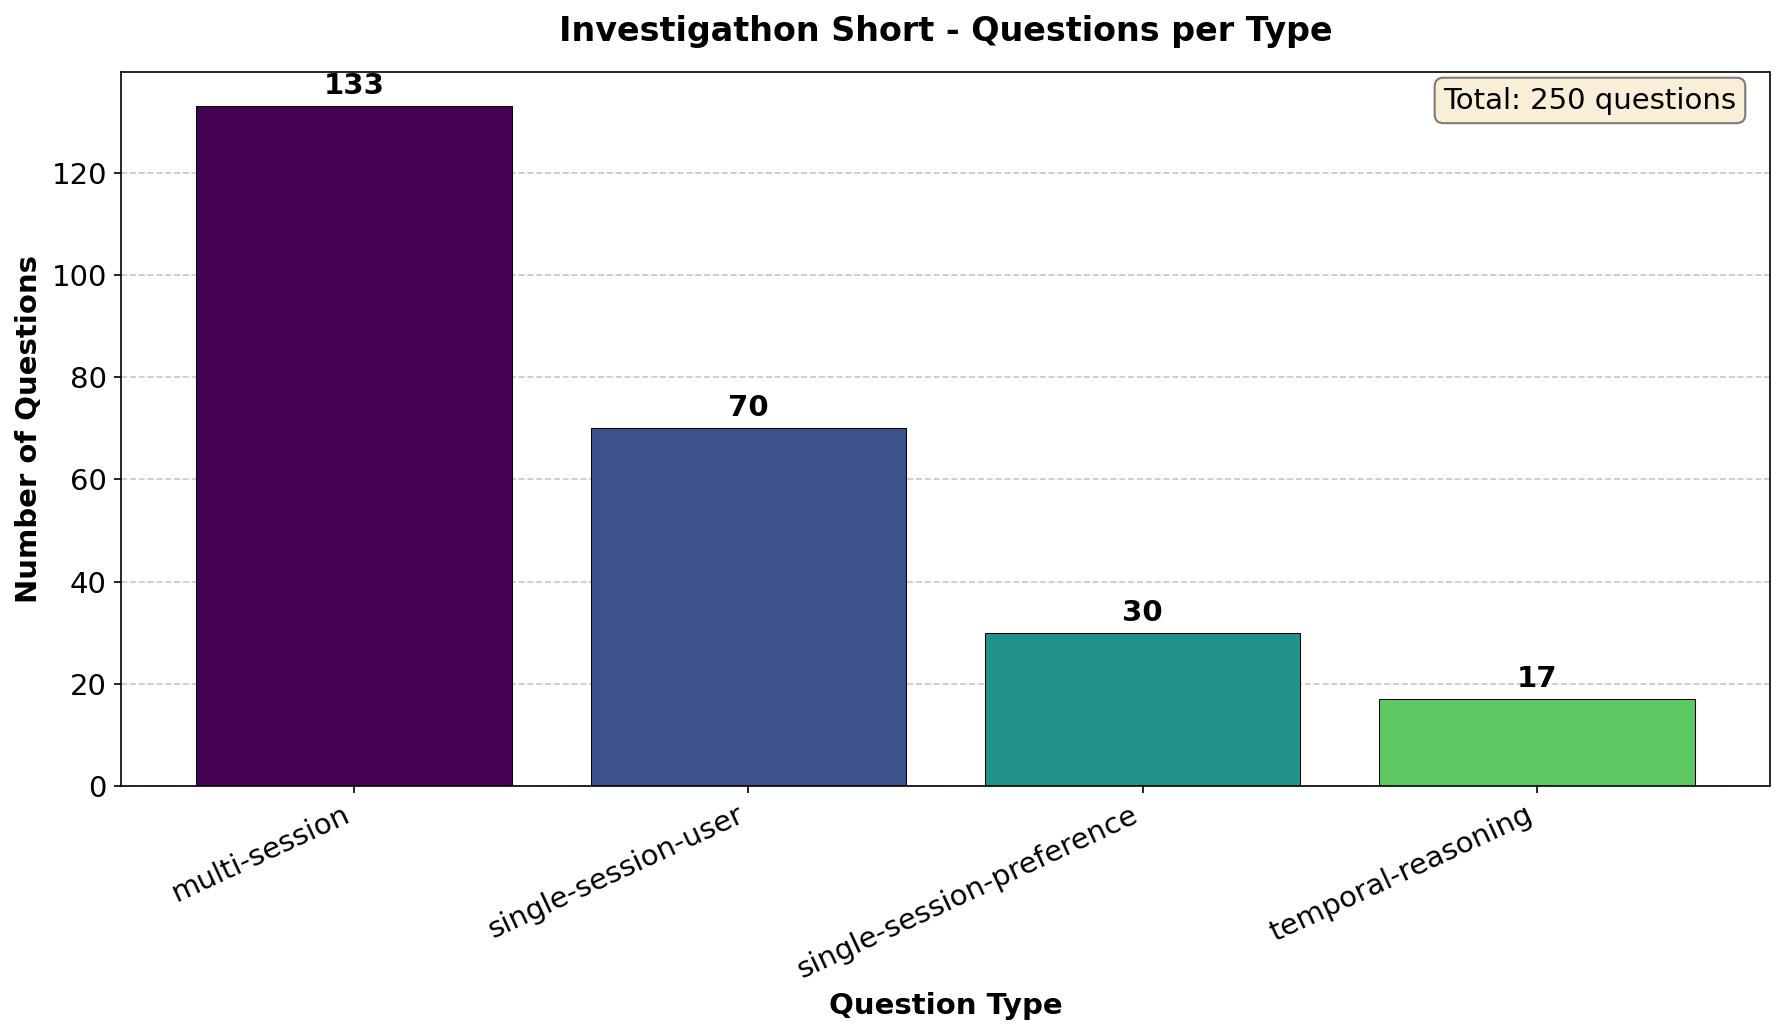
\includegraphics[width=0.48\columnwidth]{images/question_types_investigathon_short.png} 
\end{center}
}


\headerbox{Arquitectura}{name=arquitectura,column=0,below=dataset}
{
La solución se organiza en dos etapas: una offline de indexación (\textit{RAG Save}) y otra online de recuperación y generación (\textit{RAG Retrieve + LLM Generation}).

  \begin{minipage}{0.42\columnwidth}
    En la \textbf{etapa offline} el objetivo es \textbf{construir una base de conocimiento} para así poder realizar las búsquedas eficientemente en la fase online. Esta base de conocimiento se prepara en base a un historial de sesiones \texttt{s\_h}.

    Primero, a partir de un historial de sesiones, la \textit{SavePolicy} genera \textit{chunks} \texttt{[c]} y su \textit{metadata} \texttt{[m]}, se calculan los embeddings de cada chunk y se almacenan en una \textbf{base de datos vectorial}, en nuestro caso \texttt{FAISS}[3].

    En la \textbf{etapa online} el objetivo es dar una respuesta a una consulta utilizando el contexto previamente almacenado. 
    
  \end{minipage}
  \begin{minipage}{0.54\columnwidth}
    \includegraphics[width=\linewidth]{images/architecture.pdf}
  \end{minipage}

Para esto, hay una fase en la que se \textbf{obtiene la información necesaria} y luego otra en la que se \textbf{genera la respuesta}. En la primera fase, dada una \textit{pregunta} \texttt{q}, se obtiene su \textit{embedding} \texttt{e\_q}. Luego, utilizando la pregunta original y el embedding de la misma, se aplica una \textit{SearchPolicy} que va a ser la encargada de devolver los chunks y la metadata necesaria para responder a la pregunta. En la segunda fase, se genera un \textit{prompt} \texttt{p} con los datos obtenidos en la fase anterior, que se envía a la \textit{LLM}, obteniendo como resultado la \textit{respuesta final} \texttt{r}.
\\
}


\headerbox{Referencias}{name=ref,column=0,below=arquitectura,span=2}
{
{\small
\begin{minipage}{0.46\columnwidth}
\begin{enumerate}
\item P. Lewis et al. {\it Retrieval-augmented generation for knowledge-intensive NLP tasks.} NeurIPS 2024
\item D. Wu et al. {\it LongMemEval: Benchmarking Chat Assistants on Long-Term Interactive Memory.} ICLR 2024
\item M. Douze et al. {\it The FAISS Library.} IEEE Trans. on Big Data
\end{enumerate}
\end{minipage}
\begin{minipage}{0.46\columnwidth}
\begin{enumerate}
\setcounter{enumi}{3}
\item Gemma Team, Google DeepMind. {\it Gemma 3 Technical Report.} arXiv
\item J. Chen et al. {\it BGE M3-Embedding: Multi-Lingual, Multi-Functionality, Multi-Granularity Text Embeddings Through Self-Knowledge Distillation.} arXiv
\end{enumerate}
\end{minipage}
}
}


\headerbox{Resultado 1}{name=res1,column=1}
{
En el primer experimento, creamos una \textit{SavePolicy} que define un chunk por cada mensaje de cada sesión del historial de sesiones, y una \textit{SearchPolicy} que en base a la pregunta, genera el embedding de la misma y busca los 6 chunks más similares a esta. Esta versión es la más simple y es la que definimos como base.

\begin{minipage}{0.42\columnwidth}
{\small
\begin{tabular}{l r}
\hline
\textbf{Métrica} & \textbf{Valor} \\
\hline
score & 0.31 \\
online\_latency\_mean & 5.03 \\
online\_latency\_var & 2.68 \\
offline\_latency\_mean & 12.10 \\
offline\_latency\_var & 0.25 \\
context\_avg & 3253 \\
\hline
\end{tabular}
}
\end{minipage}
\begin{minipage}{0.54\columnwidth}
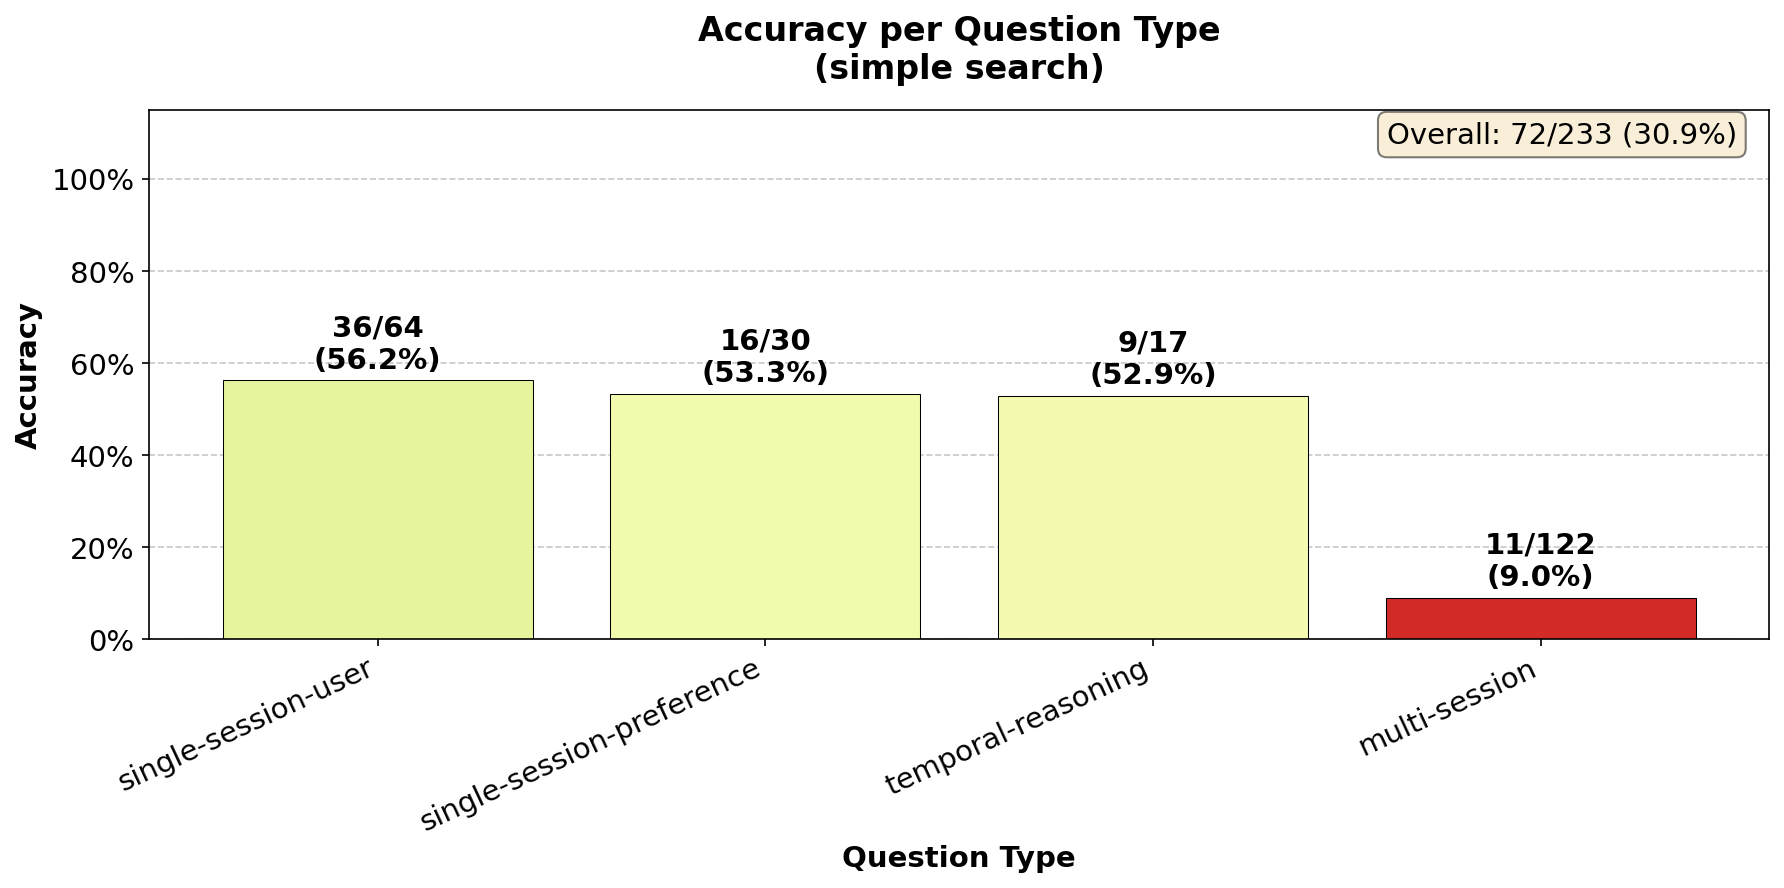
\includegraphics[width=\linewidth]{images/accuracy_SEARCH_simple_search_6_0.3.png}
\end{minipage}
}


\headerbox{Resultado 2}{name=res2,column=1,below=res1}
{
Utilizando las \textit{policies} anteriores como base, probamos dos nuevas estrategias de \textit{SearchPolicy}. La primera consiste en seleccionar más chunks en la fase de \textit{retrieve}, para luego realizar un \textbf{\textit{re-ranking}} con un modelo de embedding especializado en esta tarea. Además, realizamos otro experimento agregando \textbf{\textit{time-pruning}} para recortar sesiones fuera del rango de tiempo, pero no obtuvimos mejoras notables.

\begin{minipage}{0.42\columnwidth}
{\small
\begin{tabular}{l r}
\hline
\textbf{Métrica} & \textbf{Valor} \\
\hline
score & 0.39 \\
online\_latency\_mean & 8.19 \\
online\_latency\_var & 3.09 \\
offline\_latency\_mean & 12.15 \\
offline\_latency\_var & 0.25 \\
context\_avg & 5098 \\
\hline
\end{tabular}
}
\end{minipage}
\begin{minipage}{0.54\columnwidth}
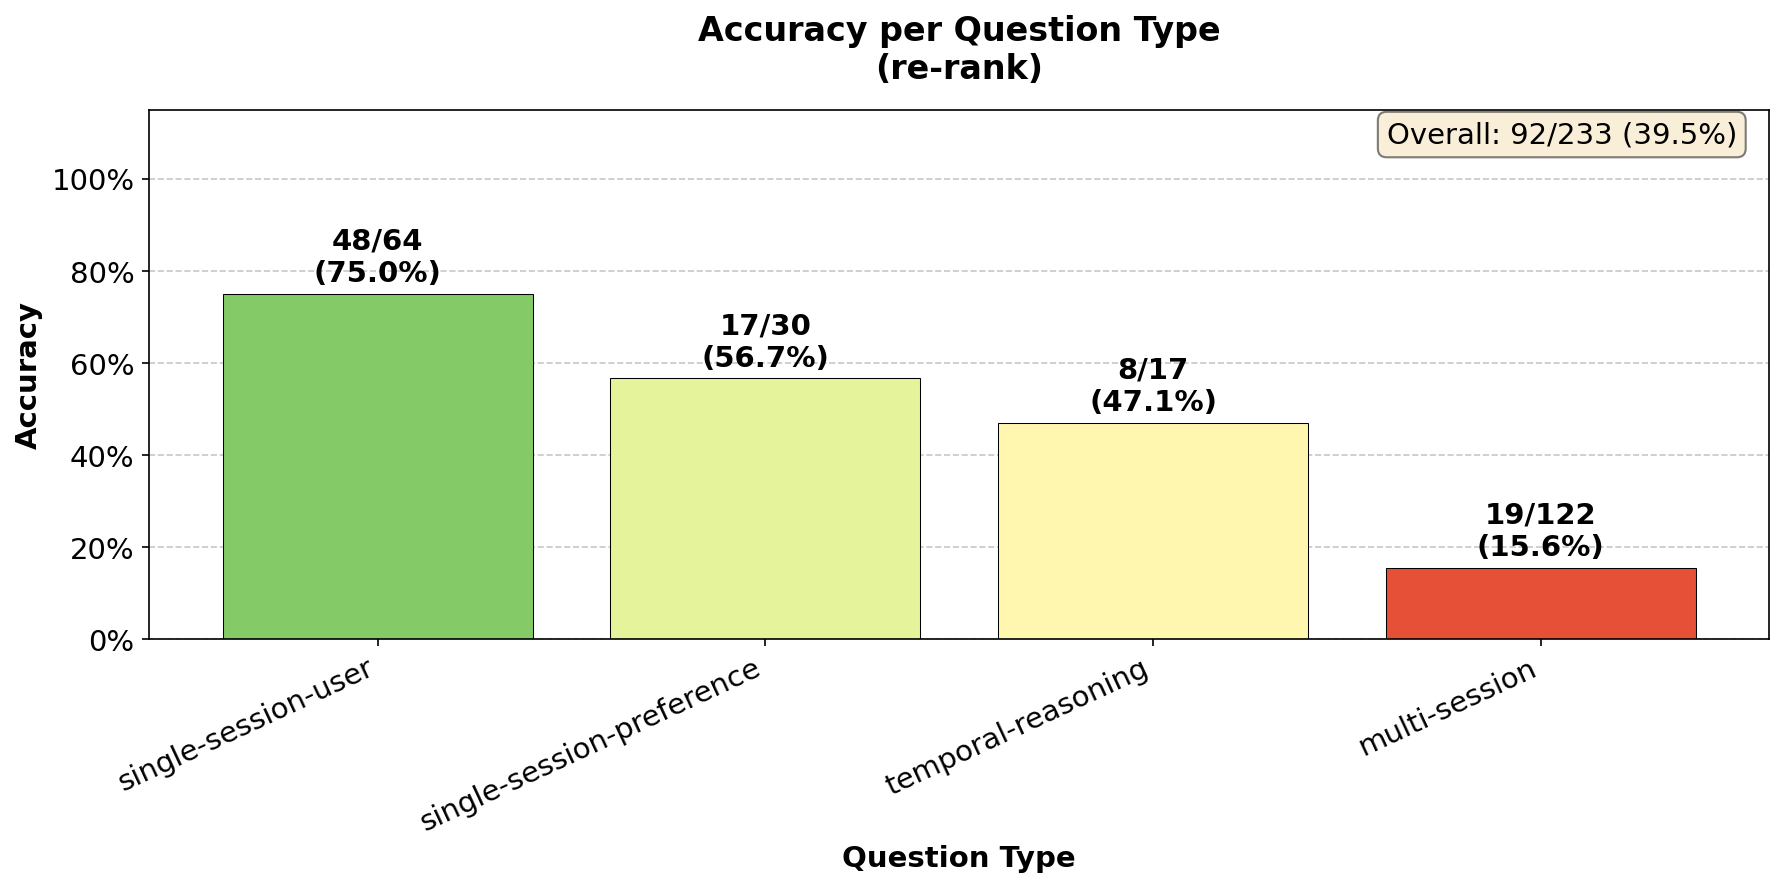
\includegraphics[width=\linewidth]{images/accuracy_SEARCH_rerank_search_BAAI_bge-reranker-v2-m3_6_0.3.png}
\end{minipage}

\begin{minipage}{0.42\columnwidth}
{\small
\begin{tabular}{l r}
\hline
\textbf{Métrica} & \textbf{Valor} \\
\hline
score & 0.38 \\
online\_latency\_mean & 8.96 \\
online\_latency\_var & 3.09 \\
offline\_latency\_mean & 12.20 \\
offline\_latency\_var & 0.26 \\
context\_avg & 4885 \\
\hline
\end{tabular}
}
\end{minipage}
\begin{minipage}{0.54\columnwidth}
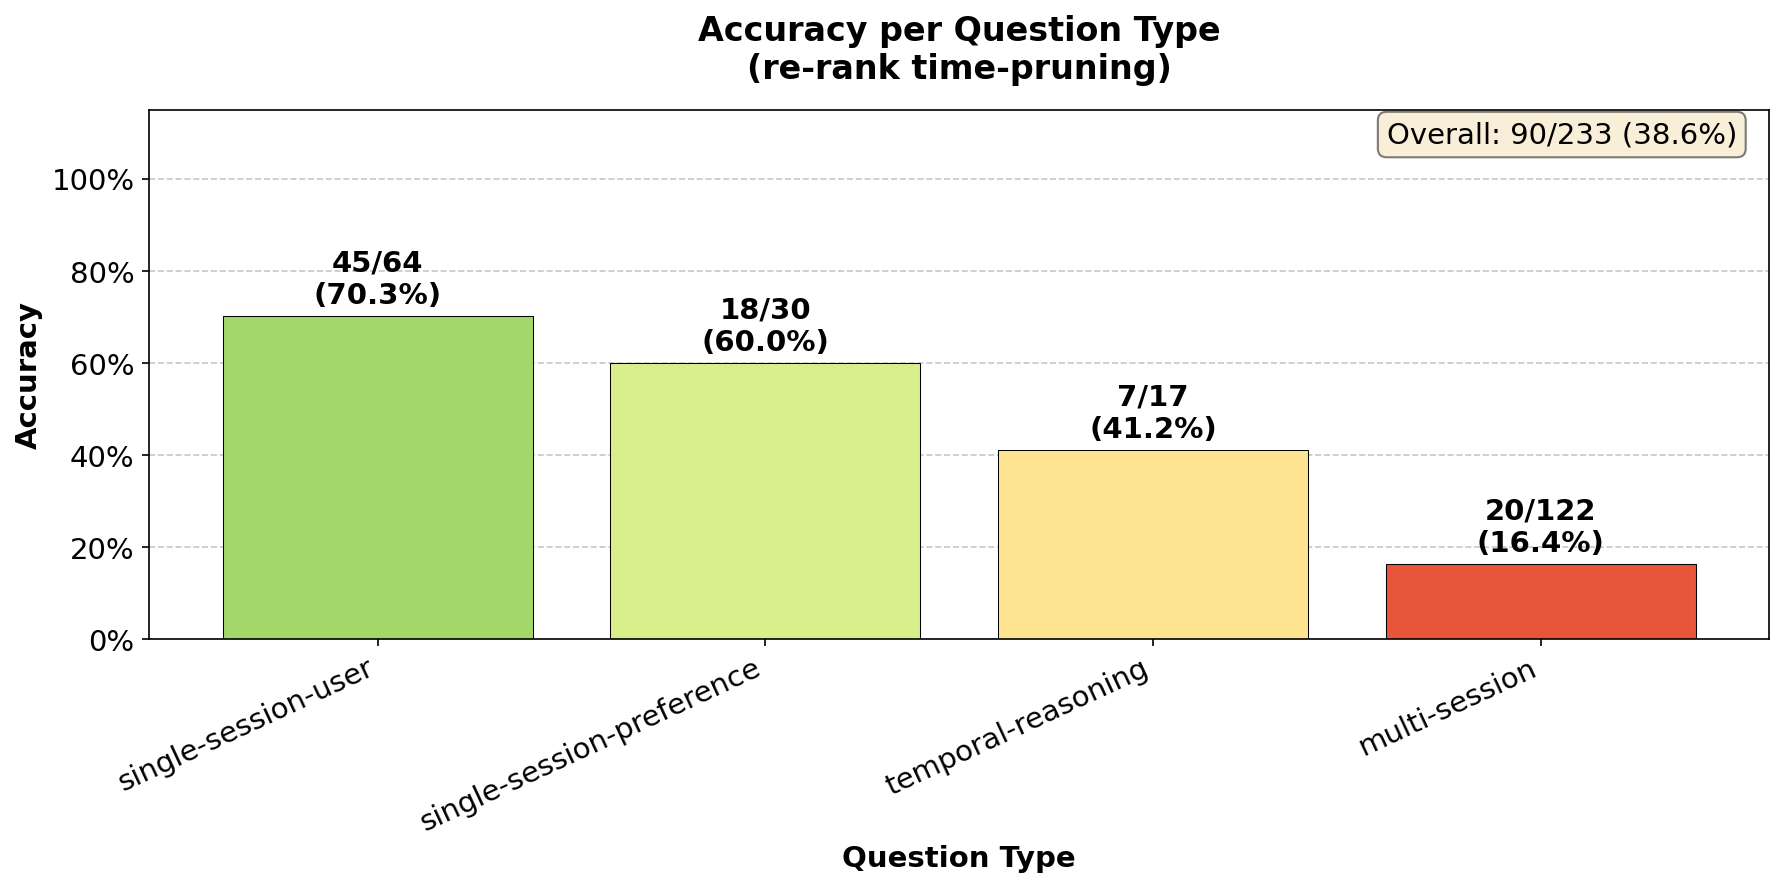
\includegraphics[width=\linewidth]{images/accuracy_SEARCH_rerank_time_pruning_search_ollama_gemma3:4b_BAAI_bge-reranker-v2-m3_6_0.3.png}
\end{minipage}
}


\headerbox{Resultado 3}{name=res3,column=1,below=res2}
{
Finalmente, descubrimos que para cada pregunta, la respuesta suele estar exclusivamente en los mensajes del usuario, o exclusivamente en los mensajes del asistente. Por lo tanto, entrenamos un \textbf{clasificador} tal que, dentro de la \textit{SearchPolicy}, primero clasifica la pregunta en si es una que debe ser contestada con los mensajes del usuario o si debe ser contestada con los mensajes del asistente. En base a esta clasificación, recuperamos solo los chunks del rol inferido a la hora de buscar en \texttt{FAISS}.

\begin{minipage}{0.42\columnwidth}
{\small
\begin{tabular}{l r}
\hline
\textbf{Métrica} & \textbf{Valor} \\
\hline
score & 0.65 \\
online\_latency\_mean & 5.28 \\
online\_latency\_var & 3.14 \\
offline\_latency\_mean & 12.19 \\
offline\_latency\_var & 0.27 \\
context\_avg & 2408 \\
\hline
\end{tabular}
}
\end{minipage}
\begin{minipage}{0.54\columnwidth}
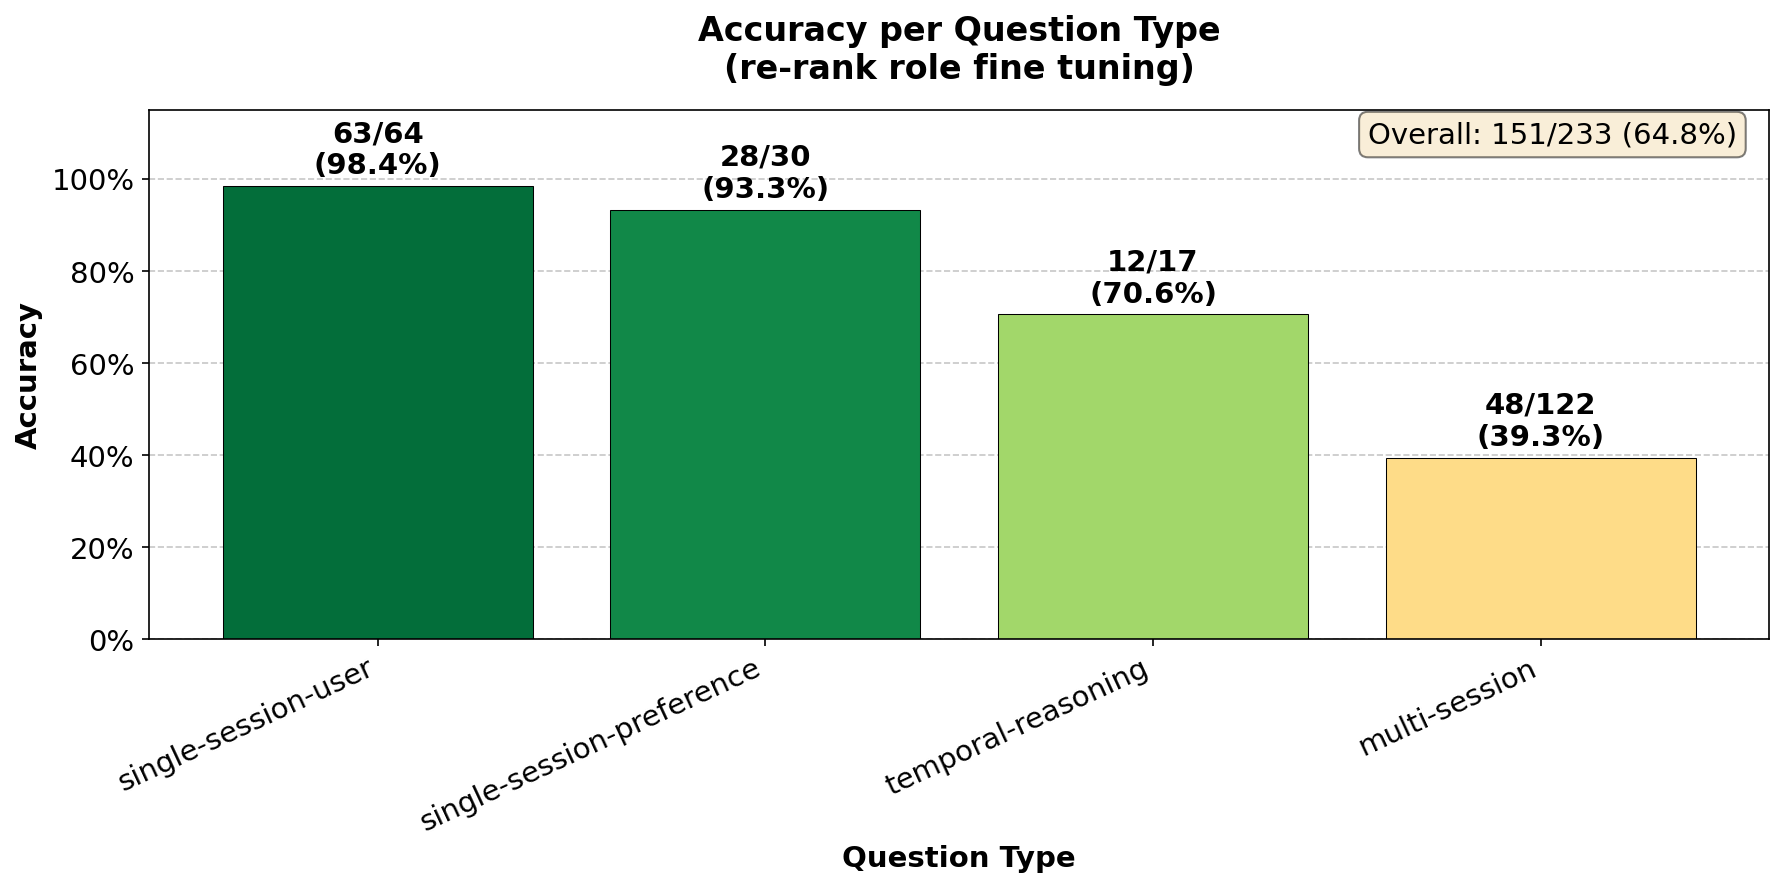
\includegraphics[width=\linewidth]{images/accuracy_SEARCH_rerank_role_search_BAAI_bge-reranker-v2-m3_fine_tuning_classifier_6_0.3.png}
\end{minipage}
}

\headerbox{Conclusión}{name=conclusion,column=1,below=res3}
{
Los resultados demuestran que las estrategias de \textit{retrieval} propuestas incrementan significativamente la relevancia de los \textit{chunks}, lo que se traduce en una mejora sustancial en la \textbf{precisión} del sistema agéntico. Dichas optimizaciones mantienen un \textbf{coste computacional marginal} sin expandir notablemente el contexto de entrada del LLM, preservando así una \textbf{baja latencia} y una \textbf{alta eficiencia}.

}

\end{poster}
\end{document}